\documentclass[notes,aspectratio=169]{beamer}
\mode<presentation>
{
  \setbeamertemplate{navigation symbols}{}
  \usetheme{ldv}
  \setbeamercovered{invisible}
  \setbeamertemplate{section in toc}[sections numbered]
  \setbeamertemplate{subsection in toc}{\leavevmode\leftskip=3.2em\rlap{\hskip-2em\inserttocsectionnumber.\inserttocsubsectionnumber}\inserttocsubsection\par}
}
\setbeameroption{show notes on second screen}

% Uncomment this if you're giving a presentation in german...
%\usepackage[ngerman]{babel}

% ...and rename this to "Folie"
\newcommand{\slidenomenclature}{Slide}
\newcommand{\warn}{\raisebox{0.325ex}{\resizebox{!}{1.2ex}{\warning}}}

\newcommand{\suc}[1]{\textcolor{green!50!black}{\emph{#1}} & \textcolor{green!50!black}{$\checkmark$} \\}
\newcommand{\fail}[1]{\textcolor{red!50!black}{\emph{#1}} & \textcolor{red!50!black}{$\times$ }\\}
\newcommand{\err}[1]{\textcolor{orange!80!black}{\emph{#1}} & \textcolor{orange!80!black}{\warning}\\}

\newcommand{\cit}[1]{\vfill\raggedleft{\parencite{#1}}}

\newcommand{\itemNote}[1]{
   \note{
      \begin{itemize}
         #1
      \end{itemize}
   }
}

\newcommand{\backupbegin}{
   \newcounter{framenumberappendix}
   \setcounter{framenumberappendix}{\value{framenumber}}
}
\newcommand{\backupend}{
   \addtocounter{framenumberappendix}{-\value{framenumber}}
   \addtocounter{framenumber}{\value{framenumberappendix}} 
}


% Add timer counters
\newcounter{SlideS}
\newcounter{SlideM}

\usepackage{ifthen}

% Command for timer and note
\newcommand{\timer}[1]{\note{S:\@#1:00\\}}

\usepackage[utf8]{inputenc}
\usepackage{amsmath,amssymb,amsfonts}
\usepackage{times}
\usepackage{graphicx}
\usepackage{fancyvrb}
\usepackage{array}
\usepackage{colortbl}
\usepackage{tabularx}

\usepackage{amssymb}
\usepackage{fourier}

\usepackage{colortbl}

\usepackage[
    type={CC},
    modifier={by},
    version={4.0},
]{doclicense}

\usepackage[style=authoryear, dashed=false]{biblatex}
\addbibresource{library.bib}

\makeatletter
\newrobustcmd*{\parentexttrack}[1]{%
  \begingroup
  \blx@blxinit
  \blx@setsfcodes
  \blx@bibopenparen#1\blx@bibcloseparen
  \endgroup}

\AtEveryCite{%
  \let\parentext=\parentexttrack%
  \let\bibopenparen=\bibopenbracket%
  \let\bibcloseparen=\bibclosebracket}
\makeatother

\usepackage[append]{beamersubframe}
\usepackage{forest}

% Uncomment me when you need to insert code
\usepackage{color}
\usepackage{listings}
% End Code

% Uncomment me when you need video or sound
\usepackage{multimedia}
\usepackage{hyperref}
% End video

% Header
\newcommand{\zwischentitel}{The Unsafety in Java RTS and Its Occurrence in the Wild}
\newcommand{\leitthema}{Lukas Döllerer}
% End Header

% Titlepage
\title{The Unsafety in Java Regression Test Selection and its Occurrence in the Wild}
\author{Lukas Döllerer}
\newcommand{\presdatum}{\today}
\institute
{
   Seminar: Software Quality\\\vspace{2mm} Informatics 4 - Software and Systems Engineering
}
% \subtitle{Sometimes we also need a subtitle}
% End Titlepage

% Slides
\begin{document}
\lstset{
   language=Java,
   basicstyle=\footnotesize \ttfamily,
   showspaces=false,
   showtabs=false,
   showstringspaces=false,
   frame=single,
   numbers=none,
   texcl=true,
   commentstyle=\color{tumcolor-green!50!black},
   keywordstyle=\color{tumcolor-blue},
   morecomment=[s][\color{tumcolor-orange!50!black}]{@}{\^^M},
}

\lstdefinestyle{highlight}{
   moredelim=**[is][\color{tumcolor-orange}]{|}{|},
}

% 1. Slide: Titlepage
\begin{frame}
   \titlepage
\end{frame}

% 2. Slide: TOC
% \begin{frame}
%    \frametitle{Table of contents}
%    \tableofcontents[subsubsectionstyle=hide]
% \end{frame}

\section{Motivation}
\begin{frame}
   \frametitle{What is the problem?}
   Over time, projects accumulate a lot of regression tests.
   \begin{columns}
      \begin{column}{0.6\textwidth}
         \begin{figure}
            \centering
            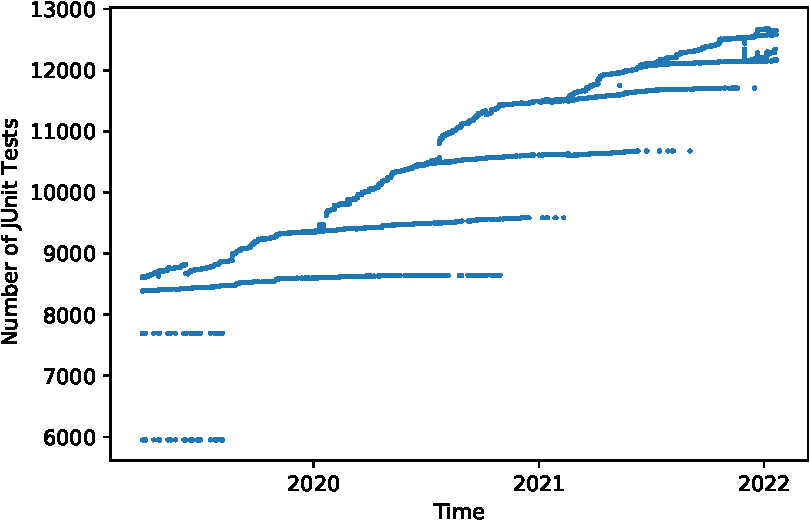
\includegraphics[scale=0.5]{./figures/pdf/junit_plot.pdf}
            \caption{Spring Boot JUnit tests in the ``master'' branch.}
         \end{figure}
      \end{column}
      \begin{column}{0.4\textwidth}
         Too many regression tests.\\\vspace{1.5mm}
         $\rightarrow$ \emph{RetestAll} not feasible\\\vspace{1.5mm}
         $\rightarrow$ \textcolor{orange!80!black}{\warn{}} Bugs / regression may be introduced.
      \end{column}
   \end{columns}
   \itemNote{
      \item Approx. number of JUnit Tests in the Spring Boot Repository.
      \item From < 9000 in Beginning 2019 to approx. 13000 now.
      \item We are assuming that these are all regression tests
      \item Test suits tend to get too big.
      \item executing all tests (called retest all) requires too many computing resources.
      \item leads to a higher probability of occuring Regression faults
   }
\end{frame}

\begin{frame}
   \frametitle{How can we solve this problem?}
   \begin{columns}[t]
      \color<2->{lightgray}{
         \begin{column}{0.3\textwidth}
            \begin{center}
               \textbf{Regression Test Minimization}
               \\\vspace*{1cm}
               Eliminate redundant test cases.
            \end{center}
         \end{column}
      }
      \color<2->{black}{
         \begin{column}{0.3\textwidth}
            \begin{center}
               \textbf{Regression Test Selection}
               \\\vspace{1cm}
               Only run affected test cases.
            \end{center}
         \end{column}
      }
      \color<2->{lightgray}{
         \begin{column}{0.3\textwidth}
            \begin{center}
               \textbf{Regression Test Prioritization}
               \\\vspace{1cm}
               Fail fast --- Maximize early fault detection.
            \end{center}
         \end{column}
      }
   \end{columns}
   \vfill\raggedleft{\textcolor<2->{lightgray}{\parencite{regression_testing_reduction}}}
   \itemNote{
      \item Yoo and Harman identified 3 ways to tackle the problem of growing regression test suites.
      \item Minimization -> Eliminate redundancy
      \item Selection -> Only execute affected tests
      \item Prioritization -> Intelligently reorder tests
      \item
      \item For today's presentation, I'm going to focus on \textbf{Regression Test Selection}.
   }
\end{frame}

\begin{frame}
   \frametitle{Regression Test Selection (RTS)}
   \begin{table}[htbp]
      \centering\begin{tabular}{l p{0.5\textwidth}}
         1. \textbf{Dependency collection:}            & Which parts of the source code affect the test's result? \\
         2. \textbf{Identification of affected tests:} & Were any of these parts changed?                         \\
      \end{tabular}
   \end{table}
   \cit{regression_testing_reduction}
   \itemNote{
      \item Regression test selection is a 2-step process
      \item 1. Dependency Collection -> Associate tests with their tested source code. (this could be done asynchronously)
      \item 2. Identification of affected tests -> Use set of source code changes to determine affected tests.
   }
   \timer{4}
\end{frame}

\begin{frame}
   \frametitle{\textbf{Safe} Regression Test Selection}
   ``[...] they select every test from the original test suite that can expose faults in the modified program.'' \parencite{safety_paper}.\\
   \vspace{1em}
   Additionally, we require that \textbf{safe} RTS does not otherwise interfere with testing.\\
   \vspace{2em}
   Since 1997, a lot of RTS tools claimed to be \textbf{safe}. However, this \emph{safety} is often only semi-formally proven for code-only changes.
   \itemNote{
      \item In 1997, two researchers defined \textbf{safe} RTS as the ability of your tool to ...
      \item We add to this definition that the rts tools must not otherwise interfere with testing.
      \item Over the last 20 years, many supposedly safe rts tools were published.
      \item Most of them do not supply perfect formal proofs of their safety. And they often only proof safety for code changes.
      \item But is this a problem?
   }
\end{frame}

\begin{frame}
   \frametitle{RTS Safety --- Not so easy?}
   Zhu and others presented \textsc{RTScheck}, a tool for testing
   RTS-Tools, in 2019.\\
   \vspace{1cm}
   They found \textbf{9 sources of unsafety} in 3 RTS-Tools that were expected to act safe in most conditions.
   \\\vspace{1cm}
   \onslide<2->{Supposedly \textbf{safe} RTS-Tools act unsafe in certain conditions.}
   \cit{unsafety_eval}
   \itemNote{
      \item In 2019, a research group published a tool called RTScheck for testing RTS-tools.
      \item First project to find empirical evidance for unsafety in supposedly safe rts tools.
      \item They found multiple sources of unsafety in popular RTS-tools.
      \item With my work, I want to extend this catalog of sources of unsafety.
   }
   \timer{4}
\end{frame}

\section{Research Questions \& Study Objects}
\begin{frame}
   \centering\Huge
   Research Questions \& \\Study Objects
\end{frame}

\newcolumntype{L}{>{\raggedright\arraybackslash}X}
\begin{frame}
   \frametitle{Study Objects}
   \begin{table}[htbp]
      \renewcommand*{\arraystretch}{2}
      \centering\begin{tabularx}{\textwidth}{| p{6em} | L | L | p{5.5em} | L | L |}
         \hline
         \textbf{Name}                                  & \emph{Ekstazi}                         & \emph{GIBstazi}                     & \emph{OpenClover}             & \emph{STARTS}          & \emph{HyRTS}                           \\
         \hline
         \small\textbf{Venue}                           & \small ISSTA                           & \small ISSRE                        & \small ---                    & \small ASE             & \small ICSE                            \\
         \hline
         \small\textbf{Dependency Collection Technique} & \small Dynamic Runtime Instrumentation & \small Dynamic with Static Analysis & \small Static Instrumentation & \small Static Analysis & \small Dynamic Runtime Instrumentation \\
         \hline
      \end{tabularx}
      \caption{Study Objects}
   \end{table}
   \nocite{ekstazimain}
   \nocite{ekstazi_tool}

   \nocite{gibstazi_paper}
   \nocite{gibstazi_tool}

   \nocite{openclover_tool}

   \nocite{starts_paper}
   \nocite{starts_tool}

   \nocite{hyrts_paper}
   \nocite{hyrts_tool}
   \itemNote{
      \item My study objects: A mix of common Java RTS-tools
      \item \textbf{Ekstazi}: Most commonly seen tool. -> International Symposium on Software Testing and Analysis
      \item \textbf{GIBstazi}: Wrapper around Ekstazi. -> International Symposium on Software Reliability Engineering
      \item \textbf{OpenClover}: Previously developed by Atlassian.
      \item \textbf{STARTS}: The only purely static tool. -> International Conference on Automated Software Engineering
      \item \textbf{HyRTS}: A hybrid RTS-tool. -> International Conference on Software Engineering
   }
   \timer{6}
\end{frame}

\begin{frame}
   \frametitle{Research Questions}
   \begin{enumerate}
      \item[RQ1] What sources of unsafety exist for the examined RTS-tools?
      \item[RQ2] What are the differences in safety of the examined tools, in the context of the previously identified sources of unsafety?
         \vspace{1.5em}
      \item[RQ3] How can potential for unsafety be automatically identified in code changes without dynamic program analysis?
      \item[RQ4] In which quantities do the identified sources of unsafety occur in real world software projects?
   \end{enumerate}
   \itemNote{
      \item Part 1: Sources of unsafety in the laboratory.
      \item[RQ1] What sources of unsafety exist for the examined RTS-tools?
      \item[RQ2] What are the differences in safety of the examined tools, in the context of the previously identified sources of unsafety?
      \item
      \item Part 2: Sources of unsafety in the wild -> look at actual software projects.
      \item[RQ3] How can potential for unsafety be automatically identified in code changes without dynamic program analysis?
      \item[RQ4] In which quantities do the identified sources of unsafety occur in real world software projects?
   }
   \timer{6}
\end{frame}

\section{Approach}
\subsection{Evaluation of Sources of Unsafety}

\begin{frame}
   \centering\Huge
   Evaluation of Sources of Unsafety\\
   \vspace{1.8cm}
   \Huge \textcolor{tumcolor-green}{RQ1 \& RQ2}
   \timer{10}
\end{frame}

\begin{subframe}
   \frametitle{Sources of Unsafety}
   \framesubtitle{Approach to Simulating Szenarios}
   Each scenario that could lead to unsafe behavior of one of the tools is simulated.
   \vspace{2mm}
   \begin{block}{Proof of Concept (PoC) Repositories}
      A \textbf{PoC Repository} contains a mini Java project that documents the steps required to reproduce the unsafe behavior.
      \\\vspace{0.5cm}
      Through Maven profiles, I can comfortably switch between tools without altering the configuration.
   \end{block}
   \itemNote{
      \item Sources of unsafety are simulated using self-sufficient Java Maven projects.
      \item They also act as a kind of documentation.
      \item For the next slides: Really quick overview over some of my identified sources of unsafety.
   }
   \timer{10}
\end{subframe}

\begin{frame}
   \frametitle{Color Code}
   \begin{columns}[b]

      \begin{column}{0.5\textwidth}
         Conflicted with the proposed source of unsafety, the RTS-tool\ldots
         \begin{table}[b]
            \renewcommand*{\arraystretch}{2}
            \begin{tabular}{|c|c|}
               \hline
               \huge\textcolor{green!50!black}{$\checkmark$} & \ldots acts \textcolor{green!50!black}{\textbf{safe}}. \\
               \hline
               \huge\textcolor{red!50!black}{$\times$}       & \ldots acts \textcolor{red!50!black}{\textbf{unsafe}}. \\
               \hline
               \huge\textcolor{orange!80!black}{\warning}    & \ldots was unable to execute the tests.                \\
               \hline
            \end{tabular}
         \end{table}
      \end{column}

      \begin{column}{0.5\textwidth}
         \centering Example:
         \begin{table}[b]
            \begin{tabular}{|c|c|}
               \hline
               \suc{Ekstazi}
               \hline
               \suc{GIBstazi}
               \hline
               \fail{OpenClover}
               \hline
               \fail{STARTS}
               \hline
               \err{HyRTS}
               \hline
            \end{tabular}
         \end{table}
      \end{column}
   \end{columns}
   \itemNote{
      \item \textbf{Important}: To find sources of unsafety, I looked at existing research, skimmed through the tool's source codes and thought about complications with the tool's dependency collection.
      \item In the following slides, you will only see the sources of unsafety that actually make one of the examined tools act unsafe.
      \item
      \item Color-Code for the following slides. -> Table on the right side of the screen. -> Table shows response of the examined tools.
      \item General notice: In order to save time, I'm not going to discuss the information contained in these tables in detail.
   }
   \timer{10}
\end{frame}

\subsubsection{Dynamic Dispatch}
\begin{subframe}
   \frametitle{Dynamic Dispatch}
   \begin{columns}[t]

      \begin{column}{0.5\textwidth}
         Runtime selection of the most specific method in the inheritance chain.
      \end{column}

      \begin{column}{0.3\textwidth}
         % \warn
         \begin{tabular}{|c|c|}
            \hline
            \suc{Ekstazi}
            \hline
            \suc{GIBstazi}
            \hline
            \fail{OpenClover}
            \hline
            \suc{STARTS}
            \hline
            \suc{HyRTS}
            \hline
         \end{tabular}
      \end{column}
   \end{columns}
   \itemNote{
      \item Question: "Does the RTS-tool act unsafe in the case of a dynamic dispatch?"
      \item As we can see, only OpenClover is not able to detect a dynamic dispatch
   }
   \timer{10}
\end{subframe}

\subsubsection{External Files}
\begin{frame}
   \frametitle{External Files}
   \vspace{4mm}
   \begin{columns}
      \begin{column}{0.5\textwidth}
         \scalebox{0.7}{
            \begin{forest}
               for tree={
               font=\ttfamily,
               grow'=0,
               child anchor=west,
               parent anchor=south,
               anchor=west,
               calign=first,
               edge path={
                     \noexpand\path [draw, \forestoption{edge}]
                     (!u.south west) +(7.5pt,0) |- node[fill,inner sep=1.25pt] {} (.child anchor)\forestoption{edge label};
                  },
               before typesetting nodes={
                     if n=1
                        {insert before={[,phantom]}}
                        {}
                  },
               fit=band,
               before computing xy={l=15pt},
               }
               [Java Project Root
                  [pom.xml]
                  [src
                        [main
                              [java
                                    [...]
                              ]
                              [\bf{resources}
                                 [...]
                              ]
                        ]
                        [test
                              [java
                                    [...]
                              ]
                              [\bf{resources}
                                 [...]
                              ]
                        ]
                  ]
                  [target]
               ]
            \end{forest}
         }
      \end{column}

      \begin{column}{0.3\textwidth}
         % \warn
         \begin{tabular}{|c|c|}
            \hline
            \fail{Ekstazi}
            \hline
            \suc{GIBstazi}
            \hline
            \fail{OpenClover}
            \hline
            \fail{STARTS}
            \hline
            \fail{HyRTS}
            \hline
         \end{tabular}
      \end{column}
   \end{columns}
   \itemNote{
      \item File resources explicitely loaded via program code.
      \item Common location for external files in maven directory structure is the resources folder.
      \item One big difference to the next source of unsafety (configuration files)
   }
   \timer{10}
\end{frame}

\subsubsection{Configuration Files}
\begin{frame}[fragile]
   \frametitle{Configuration Files}
   \vspace{4mm}
   \begin{columns}
      \begin{column}{0.5\textwidth}
         \scalebox{0.7}{
            \begin{forest}
               for tree={
               font=\ttfamily,
               grow'=0,
               child anchor=west,
               parent anchor=south,
               anchor=west,
               calign=first,
               edge path={
                     \noexpand\path [draw, \forestoption{edge}]
                     (!u.south west) +(7.5pt,0) |- node[fill,inner sep=1.25pt] {} (.child anchor)\forestoption{edge label};
                  },
               before typesetting nodes={
                     if n=1
                        {insert before={[,phantom]}}
                        {}
                  },
               fit=band,
               before computing xy={l=15pt},
               }
               [Java Project Root
                  [\bf{pom.xml}]
                  [src
                        [main
                              [java
                                    [...]
                              ]
                              [resources
                                    [...]
                              ]
                        ]
                        [test
                              [java
                                    [...]
                              ]
                              [resources
                                    [...]
                              ]
                        ]
                  ]
                  [target]
               ]
            \end{forest}
         }
      \end{column}

      \begin{column}{0.4\textwidth}
         \centering
         \begin{lstlisting}[frame=tlrb]
  <version>2.11.4</version>
\end{lstlisting}
         $\Downarrow$
         \begin{lstlisting}[frame=tlrb]
  <version>2.12.0</version>
\end{lstlisting}
         \vspace{0.3cm}
         % \warn
         \begin{tabular}{|c|c|}
            \hline
            \fail{Ekstazi}
            \hline
            \suc{GIBstazi}
            \hline
            \fail{OpenClover}
            \hline
            \suc{STARTS}
            \hline
            \fail{HyRTS}
            \hline
         \end{tabular}
      \end{column}
   \end{columns}
   \itemNote{
      \item Implicitely loaded
      \item Change behavior of libraries and external tools
      \item Here example: changing a library version
      \item ``As we can see from the response of the tools, this is actually a different source of unsafety than external files.''
   }
   \timer{10}
\end{frame}

\subsubsection{Reflections}
\begin{frame}[fragile]
   \frametitle{Reflections}
   \begin{columns}

      \begin{column}{0.5\textwidth}
         \begin{lstlisting}[frame=tlrb]
Class.forName("ModifiedClass");
\end{lstlisting}
      \end{column}

      \begin{column}{0.3\textwidth}
         % \warn
         \begin{tabular}{|c|c|}
            \hline
            \suc{Ekstazi}
            \hline
            \suc{GIBstazi}
            \hline
            \suc{OpenClover}
            \hline
            \fail{STARTS}
            \hline
            \fail{HyRTS}
            \hline
         \end{tabular}
      \end{column}
   \end{columns}
   \itemNote{
      \item A well known problem for static tools: reflections
      \item ``We focused on the \texttt{Class.forName(\ldots)} method, because it allows the programmer to access features of classes that are not explicitly imported.''
      \item Class.forname method source for most reflection problems.
   }
   \timer{10}
\end{frame}

\subsubsection{Static Initializers}
\begin{subframe}[fragile]
   \frametitle{Static Initializers}
   \begin{columns}

      \begin{column}{0.5\textwidth}
         \begin{lstlisting}[frame=tlrb]
class A {
   static {
      // Code with side-effects
   }
}

/* [...] */

Class.forName("A");
\end{lstlisting}
      \end{column}

      \begin{column}{0.3\textwidth}
         % \warn
         \begin{tabular}{|c|c|}
            \hline
            \fail{Ekstazi}
            \hline
            \fail{GIBstazi}
            \hline
            \fail{OpenClover}
            \hline
            \fail{STARTS}
            \hline
            \fail{HyRTS}
            \hline
         \end{tabular}
      \end{column}
   \end{columns}
   \timer{10}
\end{subframe}

\subsubsection{Runtime Instrumentation}
\begin{frame}[fragile]
   \frametitle{Runtime Instrumentation}
   \vspace{1em}
   \begin{columns}

      \begin{column}{0.6\textwidth}
         \textcolor{tumcolor-blue}{\emph{Ekstazi} \& \emph{GIBstazi}:}\\
         \small{Dynamic Bytecode Instrumentation incompatible with modern language features.}
         \begin{lstlisting}[frame=tlrb]
MyClass.class.getAnnotatedInterfaces();
MyClass.class.toGenericString();
         \end{lstlisting}
         \vspace{1.5em}
         \textcolor{tumcolor-blue}{\emph{OpenClover}:}\\
         \small{Source Code Instrumentation alters results of reflective method calls.}
         \begin{lstlisting}[frame=tlrb]
MyClass.class.getDeclaredClasses();
MyClass.class.getFields();
         \end{lstlisting}
      \end{column}

      \begin{column}{0.3\textwidth}
         % \warn
         \begin{tabular}{|c|c|}
            \hline
            \fail{Ekstazi}
            \hline
            \fail{GIBstazi}
            \hline
            \fail{OpenClover}
            \hline
            \suc{STARTS}
            \hline
            \suc{HyRTS}
            \hline
         \end{tabular}
      \end{column}
   \end{columns}
   \itemNote{
      \item Special source of unsafety:
      \item A rather common problem - Runtime instrumentation that changes the code's behavior
      \item Invasive or buggy runtime instrumentation can cause unsafety.
      \item Ekstazi's and GIBstazi's (Dynamic Bytecode Instrumentation) can't execute all reflective method calls, which is causing runtime errors
      \item OpenClover's source code instrumentation adds fields and classes and therefore secretly changes method call results.
   }
   \timer{10}
\end{frame}

\begin{subframe}
   \frametitle{Runtime Instrumentation}
   \framesubtitle{Keywords that cause unsafety.}
   \begin{table}[H]
      \centering
      \begin{tabular}{l | l}
         \hline
         \emph{Ekstazi}                    & \emph{OpenClover}             \\
         \hline
         \texttt{getAnnotatedInterfaces()} & \texttt{getDeclaredClasses()} \\
         \texttt{getAnnotatedSuperclass()} & \texttt{getDeclaredFields()}  \\
         \texttt{toGenericString()}        & \texttt{getClasses()}         \\
                                           & \texttt{getFields()}          \\
      \end{tabular}
      \caption{Methods whose behavior changes with the corresponding RTS-tools runtime
         instrumentation. All methods are called on the meta class object of type \nolinkurl{Class}.}
   \end{table}
\end{subframe}

\subsubsection{Dependency Injection}
\begin{subframe}
   \frametitle{Dependency Injection}
   \begin{columns}[t]
      \begin{column}{0.3\textwidth}
         Examined Frameworks:
         \begin{itemize}
            \item Spring
            \item Guice
         \end{itemize}
      \end{column}
      \begin{column}{0.6\textwidth}
         Scenarios:
         \begin{itemize}
            \item Configuration in External File
            \item Configuration in Code
                  \begin{itemize}
                     \item Dependency Source Code Changes
                     \item Collection Injection
                     \item Implicit Configuration\\$\Rightarrow$ Class Path Scanning (Spring-only)
                  \end{itemize}
         \end{itemize}
      \end{column}
   \end{columns}
   \timer{10}
\end{subframe}

\subsubsection{Configuration in External Files}
\begin{subframe}
   \frametitle{Dependency Injection}
   \framesubtitle{Configuration in External Files}
   \begin{columns}
      \begin{column}{0.6\textwidth}
         When placing the configuration of dependencies into an external file, the primary cause of unsafety is the tool's
         inability to detect changes to this external file.
      \end{column}

      \begin{column}{0.3\textwidth}
         % \warn
         \begin{tabular}{|c|c|}
            \hline
            \fail{Ekstazi}
            \hline
            \suc{GIBstazi}
            \hline
            \fail{OpenClover}
            \hline
            \fail{STARTS}
            \hline
            \fail{HyRTS}
            \hline
         \end{tabular}
      \end{column}
   \end{columns}
   \timer{10}
\end{subframe}

\subsubsection{Dependency Source Code Changes - Spring Framework}
\begin{frame}[fragile]
   \frametitle{Dependency Injection (1/3)}
   \framesubtitle{Dependency Source Code Changes - Spring Framework}
   \begin{columns}
      \begin{column}{0.5\textwidth}
         \begin{lstlisting}[frame=tlrb]
@Bean
public BeanInterface beanName() {
   // change this implementation
   return new Implementation(); 
}
\end{lstlisting}
      \end{column}

      \begin{column}{0.3\textwidth}
         % \warn
         \begin{tabular}{|c|c|}
            \hline
            \suc{Ekstazi}
            \hline
            \err{GIBstazi}
            \hline
            \err{OpenClover}
            \hline
            \fail{STARTS}
            \hline
            \suc{HyRTS}
            \hline
         \end{tabular}
      \end{column}
   \end{columns}
   \itemNote{
      \item Probably one of the most underestimated sources of unsafety.
      \item Once dependency injection is applied, the examined tools start to act unsafely
      \item Focused research on Spring and Guice frameworks as they are the most commonly used libraries.
      \item
      \item For starters, this is a straight forward source of unsafety:
      \item Declare an injected dependency, create a matching implementation and change this implementation. (here with Spring)
      \item -> next slide for Guice
   }
   \timer{10}
\end{frame}

\subsubsection{Dependency Source Code Changes - Guice Framework}
\begin{frame}[fragile]
   \frametitle{Dependency Injection (1/3)}
   \framesubtitle{Dependency Source Code Changes - Guice Framework}
   \begin{columns}
      \begin{column}{0.5\textwidth}
         \begin{lstlisting}[frame=tlrb]
@ImplementedBy(A.class)
public interface InterfaceA {
      void method();
}

class A {
   // change this source code
}
\end{lstlisting}
      \end{column}

      \begin{column}{0.3\textwidth}
         % \warn
         \begin{tabular}{|c|c|}
            \hline
            \suc{Ekstazi}
            \hline
            \suc{GIBstazi}
            \hline
            \suc{OpenClover}
            \hline
            \fail{STARTS}
            \hline
            \suc{HyRTS}
            \hline
         \end{tabular}
      \end{column}
   \end{columns}
   \itemNote{
      \item Change the implementation of an injected dependency with Guice.
   }
   \timer{10}
\end{frame}

\subsubsection{Collection Injection - Spring Framework}
\begin{frame}[fragile]
   \frametitle{Dependency Injection (2/3)}
   \framesubtitle{Collection Injection - Spring Framework}
   \begin{columns}
      \begin{column}{0.55\textwidth}
         \begin{lstlisting}[frame=tlrb]
@Autowired
Collection<BeanInterface> injected;
\end{lstlisting}

         $\Rightarrow$ Multiple Beans packed into a collection.
      \end{column}

      \begin{column}{0.3\textwidth}
         % \warn
         \begin{tabular}{|c|c|}
            \hline
            \fail{Ekstazi}
            \hline
            \err{GIBstazi}
            \hline
            \err{OpenClover}
            \hline
            \fail{STARTS}
            \hline
            \fail{HyRTS}
            \hline
         \end{tabular}
      \end{column}
   \end{columns}
   \itemNote{
      \item Big problem with the Spring framework: Automatic classpath scanning (we'll come back to that in a moment)
      \item Define multiple implementations for the same dependency (Bean) -> Spring \emph{implictly} packs all into a collection
      \item Adding new implementations is undetected
   }
   \timer{10}
\end{frame}

\subsubsection{Collection Injection - Guice Framework}
\begin{frame}[fragile]
   \frametitle{Dependency Injection (2/3)}
   \framesubtitle{Collection Injection - Guice Framework}
   \begin{columns}
      \begin{column}{0.5\textwidth}
         \begin{lstlisting}[frame=tlrb]
@ProvidesIntoSet
InjectedType impl1() {
   return Implementation();
}

@ProvidesIntoSet
InjectedType impl2() {
   return OtherImplementation();
}
\end{lstlisting}

         $\Rightarrow$ Set of multiple implementations.
      \end{column}

      \begin{column}{0.3\textwidth}
         % \warn
         \begin{tabular}{|c|c|}
            \hline
            \suc{Ekstazi}
            \hline
            \suc{GIBstazi}
            \hline
            \suc{OpenClover}
            \hline
            \suc{STARTS}
            \hline
            \fail{HyRTS}
            \hline
         \end{tabular}
      \end{column}
   \end{columns}
   \itemNote{
      \item Collection injection is also available for the Guice framework
      \item way more \emph{explicit}
      \item Most tools are quite good at detecting Guice collection injection.
   }
   \timer{10}
\end{frame}

\subsubsection{Classpath Scanning}
\begin{frame}[fragile]
   \frametitle{Dependency Injection (3/3)}
   \framesubtitle{Classpath Scanning - Spring Framework only}
   \begin{columns}
      \begin{column}{0.5\textwidth}
         \begin{lstlisting}[frame=tlrb]
@SpringBootApplication
public class MainSpringAppClass { }

@Configuration
@ComponentScan("example.beanConfig")
public class MainConfiguration { }
\end{lstlisting}
      \end{column}

      \begin{column}{0.3\textwidth}
         % \warn
         \begin{tabular}{|c|c|}
            \hline
            \fail{Ekstazi}
            \hline
            \textcolor{red!50!black}{\emph{GIBstazi}}   & \textcolor{red!50!black}{$\times$} /  \textcolor{orange!80!black}{\warning} \\
            \hline
            \textcolor{red!50!black}{\emph{OpenClover}} & \textcolor{red!50!black}{$\times$} /  \textcolor{orange!80!black}{\warning} \\
            \hline
            \fail{STARTS}
            \hline
            \fail{HyRTS}
            \hline
         \end{tabular}
      \end{column}
   \end{columns}
   \itemNote{
      \item Classpath scanning - the big source of unsafety of the spring framework
      \item The code only uses annotations and doesn't explicitely call an injector or configuration class.
      \item Spring handles dependency management in the background
      \item -> Dependencies are unclear, changes may not be detected
   }
   \timer{10}
\end{frame}

\subsection{Occurence of Unsafety in the Wild}

\begin{frame}
   \centering\Huge
   Occurence of Unsafety in the Wild\\
   \vspace{1.8cm}
   \Huge \textcolor{tumcolor-green}{RQ3 \& RQ4}
   \timer{13}
\end{frame}

\begin{frame}
   \frametitle{Occurence in the Wild}

   \large But, are these scenarios actually relevant?\\
   \vspace{0.8cm}
   \large Do these sources of unsafety occur in real-world software projects?\\
   \vspace{1.5cm}
   $\Rightarrow$ Search through the last 100 commits of 100 open source projects.
   \itemNote{
      \item You may ask yourselfs: ``Are these purely hypothetical sources of unsafety that occur under laboratory conditions?''
      \item I askes myself the same question.
      \item Performed a broad search.
   }
   \timer{13}
\end{frame}

\begin{frame}
   \frametitle{Occurence in the Wild}
   \framesubtitle{Study Object Selection}
   Choose the 100 public projects with the most ``stars'' from GitHub that\ldots
   \vspace{0.2cm}
   \begin{itemize}
      \item \ldots have the majority of their code written in Java
      \item \ldots use Maven as their build system
      \item \ldots were recently updated (at least once after the 06/01/2020)
      \item \ldots have at least 100 JUnit test cases (approximated)
      \item \ldots
   \end{itemize}
   \itemNote{
      \item Filtered the most popular open source repositories from github
      \item They had to be mostly written in Java, use Maven und were recently updated.
      \item[+] They need to have at least 100 Junit tests
      \item[->] we want to make sure that the projects are actual candidates for using an RTS solution in the future
      \item We sorted all these repositories by stars and picked the top 100 to be our study objects.
   }
   \timer{13}
\end{frame}

\begin{frame}
   \frametitle{Occurence in the Wild}
   \framesubtitle{Study Object Selection}

   A selection of the contained projects. \small{(Collected between 11/11/2021 and 11/13/2021)}
   \begin{columns}[t]
      \begin{column}{0.4\textwidth}
         \begin{itemize}
            \item Google Guava (42835 Stars)
            \item Apache Dubbo (36435 Stars)
            \item Jenkins (18057 Stars)
            \item Apache Flink (17519 Stars)
            \item Apache Hadoop (12081 Stars)
         \end{itemize}
      \end{column}
      \begin{column}{0.5\textwidth}
         \begin{itemize}
            \item Google Guice (10532 Stars)
            \item Apache Zookeeper (9962 Stars)
            \item JUnit 4 (8213 Stars)
            \item Signalapp Signal-Server (7210 Stars)
            \item Apache HBase (4260 Stars)
         \end{itemize}
      \end{column}
   \end{columns}
   \itemNote{
      \item Only a quick overview over some of the well known projects in the study object group.
   }
   \timer{13}
\end{frame}

\begin{frame}
   \frametitle{Occurence in the Wild}
   \framesubtitle{Commit Scanners}
   \vspace{0.2cm}
   Scan of the last 100 commits of each project. Each source of unsafety was evaluated based on these questions.
   \begin{table}[htbp]
      \renewcommand*{\arraystretch}{1.4}
      \centering\begin{tabularx}{\textwidth}{|L|L|L|L|}
         \hline
         \textbf{External Files}                             & \textbf{Dependency Injection}                                            & \textbf{Runtime Instrumentation}                              & \textbf{Reflections}                                                                                  \\
         \hline
         \small{Did the commiter change any external files?} & \small{Was any keyword related to dependency injection added / removed?} & \small{Does the source code contain any problematic methods?} & \small{1. Were reflective accesses introduced?\newline2. Were reflectively accessed classes changed?} \\
         \hline
      \end{tabularx}
      \caption{Commit Scanner Objectives}
   \end{table}
   \itemNote{
      \footnotesize
      \item To detect said sources of unsafety, I created, what I call, "commit scanners".
      \item
      \item External files scanner: detectes commit changes to files in the resources folder (maven, previously shown)
      \item Dependency Injection scanner: Searches for keywords that are related to spring or guice dependency injection and might introduce unsafety
      \item Runtime Instrumentation scanner: Detects keywords that cause unsafety with the runtime instrumentation of some of the examined tools.
      \item Reflections Scanner: Detects occurences of the \texttt{Class.forName(...)} method call
      \item Reflections Scanner: Also searches for changes on classes that are reflectively accessed
      \item \textcolor{gray}{Reflections Scanner: Detected reflections also trigger static initializers -> more yield}
      \item I'm not going to go into technical details of the scanning and jump right to the results.
   }
   \timer{13}
\end{frame}

\begin{frame}[fragile]
   \frametitle{Commit Scanners --- Pseudocode}
   Main Repository Scanner:
   \begin{lstlisting}[frame=tlrb, language=Python]
for commit in repo.traverse_commits(to=100):
   for scanner in commit_scanners:
         scanner.scan(commit)
   \end{lstlisting}
   \vspace{1em}
   Commit Scanner Module:
   \begin{lstlisting}[frame=tlrb, language=Python, style=highlight]
def scan(self, commit):
   for change in commit:
      if |change_is_source_of_unsafety(change)|:
         self.unsafety_storage.add(commit)
   \end{lstlisting}
\end{frame}

\section{Results}

\begin{frame}
   \centering\Huge
   Results
   \timer{17}
\end{frame}

\begin{frame}
   \frametitle{Results}
   \framesubtitle{Sources of Unsafety for specific RTS-Tools: RQ1 \& RQ2}
   \begin{table}[h]
      \centering %TODO: schlimme Zeilen hervorheben
      \resizebox*{\textwidth}{!}{
         \begin{tabular}{|l | c | c | c | c | c|}
            \hline
            Source of Unsafety                    & \emph{Ekstazi}                           & \emph{GIBstazi}                          & \emph{OpenClover}                        & \emph{STARTS}                            & \emph{HyRTS}                             \\
            \hline
            \textcolor{gray}{Dynamic Dispatch}    & \textcolor{green!50!black}{$\checkmark$} & \textcolor{green!50!black}{$\checkmark$} & \textcolor{red!50!black}{$\times$ }      & \textcolor{green!50!black}{$\checkmark$} & \textcolor{green!50!black}{$\checkmark$} \\
            External Files                        & \textcolor{red!50!black}{$\times$ }      & \textcolor{green!50!black}{$\checkmark$} & \textcolor{red!50!black}{$\times$ }      & \textcolor{red!50!black}{$\times$ }      & \textcolor{red!50!black}{$\times$ }      \\
            Configuration Files                   & \textcolor{red!50!black}{$\times$ }      & \textcolor{green!50!black}{$\checkmark$} & \textcolor{red!50!black}{$\times$ }      & \textcolor{green!50!black}{$\checkmark$} & \textcolor{red!50!black}{$\times$ }      \\
            Reflections                           & \textcolor{green!50!black}{$\checkmark$} & \textcolor{green!50!black}{$\checkmark$} & \textcolor{green!50!black}{$\checkmark$} & \textcolor{red!50!black}{$\times$ }      & \textcolor{red!50!black}{$\times$ }      \\
            \textcolor{gray}{Static Initializers} & \textcolor{red!50!black}{$\times$ }      & \textcolor{red!50!black}{$\times$ }      & \textcolor{red!50!black}{$\times$ }      & \textcolor{red!50!black}{$\times$ }      & \textcolor{red!50!black}{$\times$ }      \\
            Dependency Injection (Spring)         & \textcolor{green!50!black}{$\checkmark$} & \textcolor{orange!80!black}{\warn}       & \textcolor{orange!80!black}{\warn}       & \textcolor{red!50!black}{$\times$ }      & \textcolor{green!50!black}{$\checkmark$} \\
            Dependency Injection (Guice)          & \textcolor{green!50!black}{$\checkmark$} & \textcolor{green!50!black}{$\checkmark$} & \textcolor{green!50!black}{$\checkmark$} & \textcolor{red!50!black}{$\times$ }      & \textcolor{green!50!black}{$\checkmark$} \\
            Collection Injection (Spring)         & \textcolor{red!50!black}{$\times$ }      & \textcolor{orange!80!black}{\warn}       & \textcolor{orange!80!black}{\warn}       & \textcolor{red!50!black}{$\times$ }      & \textcolor{red!50!black}{$\times$ }      \\
            Collection Injection (Guice)          & \textcolor{green!50!black}{$\checkmark$} & \textcolor{green!50!black}{$\checkmark$} & \textcolor{green!50!black}{$\checkmark$} & \textcolor{green!50!black}{$\checkmark$} & \textcolor{red!50!black}{$\times$ }      \\
            Classpath Scanning (Spring)           & \textcolor{red!50!black}{$\times$ }      & \textcolor{red!50!black}{$\times$ }      & \textcolor{red!50!black}{$\times$ }      & \textcolor{red!50!black}{$\times$ }      & \textcolor{red!50!black}{$\times$ }      \\
            Runtime Instrumentation               & \textcolor{red!50!black}{$\times$ }      & \textcolor{red!50!black}{$\times$ }      & \textcolor{red!50!black}{$\times$ }      & \textcolor{green!50!black}{$\checkmark$} & \textcolor{green!50!black}{$\checkmark$} \\
            \hline
         \end{tabular}
      }
      \caption{Test results from the PoC Repositories.}
   \end{table}
   \itemNote{
      \item Full evaluation of the discovered sources of unsafety. (same color code as before)
      \item The gray sources weren't previously discussed
      \item
      \item Few things to note:\begin{itemize}
         \item External files are only safe with GIBstazi
         \item static initialization, spring dependency injection and classpath scanning is unsafe with all examined tools
      \end{itemize}
      \item following are the results of the scans of real world software projects.
   }
   \timer{17}
\end{frame}

\begin{frame}
   \frametitle{Results}
   \framesubtitle{Sources of Unsafety for specific RTS-Tools: RQ1 \& RQ2}
   \begin{table}[h]
      \centering %TODO: schlimme Zeilen hervorheben
      \resizebox*{\textwidth}{!}{
         \begin{tabular}{|l | c | c | c | c | c|}
            \hline
            Source of Unsafety                 & \emph{Ekstazi}                           & \emph{GIBstazi}                          & \emph{OpenClover}                        & \emph{STARTS}                            & \emph{HyRTS}                             \\
            \hline
            \textcolor{gray}{Dynamic Dispatch} & \textcolor{green!50!black}{$\checkmark$} & \textcolor{green!50!black}{$\checkmark$} & \textcolor{red!50!black}{$\times$ }      & \textcolor{green!50!black}{$\checkmark$} & \textcolor{green!50!black}{$\checkmark$} \\
            \rowcolor{red!20!white}
            External Files                     & \textcolor{red!50!black}{$\times$ }      & \textcolor{green!50!black}{$\checkmark$} & \textcolor{red!50!black}{$\times$ }      & \textcolor{red!50!black}{$\times$ }      & \textcolor{red!50!black}{$\times$ }      \\
            Configuration Files                & \textcolor{red!50!black}{$\times$ }      & \textcolor{green!50!black}{$\checkmark$} & \textcolor{red!50!black}{$\times$ }      & \textcolor{green!50!black}{$\checkmark$} & \textcolor{red!50!black}{$\times$ }      \\
            Reflections                        & \textcolor{green!50!black}{$\checkmark$} & \textcolor{green!50!black}{$\checkmark$} & \textcolor{green!50!black}{$\checkmark$} & \textcolor{red!50!black}{$\times$ }      & \textcolor{red!50!black}{$\times$ }      \\
            \rowcolor{red!20!white}
            Static Initializers                & \textcolor{red!50!black}{$\times$ }      & \textcolor{red!50!black}{$\times$ }      & \textcolor{red!50!black}{$\times$ }      & \textcolor{red!50!black}{$\times$ }      & \textcolor{red!50!black}{$\times$ }      \\
            Dependency Injection (Spring)      & \textcolor{green!50!black}{$\checkmark$} & \textcolor{orange!80!black}{\warn}       & \textcolor{orange!80!black}{\warn}       & \textcolor{red!50!black}{$\times$ }      & \textcolor{green!50!black}{$\checkmark$} \\
            Dependency Injection (Guice)       & \textcolor{green!50!black}{$\checkmark$} & \textcolor{green!50!black}{$\checkmark$} & \textcolor{green!50!black}{$\checkmark$} & \textcolor{red!50!black}{$\times$ }      & \textcolor{green!50!black}{$\checkmark$} \\
            \rowcolor{red!20!white}
            Collection Injection (Spring)      & \textcolor{red!50!black}{$\times$ }      & \textcolor{orange!80!black}{\warn}       & \textcolor{orange!80!black}{\warn}       & \textcolor{red!50!black}{$\times$ }      & \textcolor{red!50!black}{$\times$ }      \\
            Collection Injection (Guice)       & \textcolor{green!50!black}{$\checkmark$} & \textcolor{green!50!black}{$\checkmark$} & \textcolor{green!50!black}{$\checkmark$} & \textcolor{green!50!black}{$\checkmark$} & \textcolor{red!50!black}{$\times$ }      \\
            \rowcolor{red!20!white}
            Classpath Scanning (Spring)        & \textcolor{red!50!black}{$\times$ }      & \textcolor{red!50!black}{$\times$ }      & \textcolor{red!50!black}{$\times$ }      & \textcolor{red!50!black}{$\times$ }      & \textcolor{red!50!black}{$\times$ }      \\
            Runtime Instrumentation            & \textcolor{red!50!black}{$\times$ }      & \textcolor{red!50!black}{$\times$ }      & \textcolor{red!50!black}{$\times$ }      & \textcolor{green!50!black}{$\checkmark$} & \textcolor{green!50!black}{$\checkmark$} \\
            \hline
         \end{tabular}
      }
      \caption{Test results from the PoC Repositories.}
   \end{table}
   \itemNote{
      \item Full evaluation of the discovered sources of unsafety. (same color code as before)
      \item The gray sources weren't previously discussed
      \item
      \item Few things to note:\begin{itemize}
         \item External files are only safe with GIBstazi
         \item static initialization, spring dependency injection and classpath scanning is unsafe with all examined tools
      \end{itemize}
      \item following are the results of the scans of real world software projects.
   }
   \timer{17}
\end{frame}

\begin{frame}
   \frametitle{Results}
   \framesubtitle{Occurence of Sources of Unsafety in the Wild: RQ3 \& RQ4}
   \begin{table}[h]
      \centering
      \renewcommand*{\arraystretch}{1.4}
      \begin{tabularx}{\textwidth}{|L|}
         \hline
         \textbf{External Files Scanner}                                                              \\
         \hline
         \begin{itemize}
            \setlength\itemsep{1em}
            \item 10\% of the scanned commits change external files.
            \item They alter, on average, 1993.59 lines of text in an average of 11.85 files.
            \item These changes were only counted in the \texttt{resources} and \texttt{filters} folders.
         \end{itemize} \\
         \hline
      \end{tabularx}
   \end{table}
   \itemNote{
      \item starting with the external files scanner:
      \item 989 scanned commits have potential for unsafety
      \item We detected big changes to a lot of external files, making this an important factor to safety.
   }
   \timer{17}
\end{frame}


\begin{frame}
   \frametitle{Results}
   \framesubtitle{Occurence of Sources of Unsafety in the Wild: RQ3 \& RQ4}
   \begin{table}[h]
      \centering
      \renewcommand*{\arraystretch}{1.4}
      \begin{tabularx}{\textwidth}{|L|}
         \hline
         \textbf{Dependency Injection}                                                 \\
         \hline
         \begin{itemize}
            \setlength\itemsep{1em}
            \item 53\% of the projects use the Spring framework, 17\% use Guice libraries.
            \item Detected 484 commits with Spring-related changes
            \item \ldots and 297 commits with Guice-related changes.
         \end{itemize} \\
         \hline
      \end{tabularx}
   \end{table}
   \itemNote{
      \item Dependency injection is very important: the majority of the scanned projects uses the spring framework and 17\% use guice
      \item Detected potential for unsafety in 484 commits for spring and 297 commits for guice
      \item This has to be evaluated even further, but automatically classifying these is hard.
   }
   \timer{17}
\end{frame}

\begin{subframe}[fragile=singleslide]
   \frametitle{Keywords for Dependency Injections}
   \framesubtitle{Occurence of Sources of Unsafety in the Wild: RQ3 \& RQ4}
   \begin{table}[h]
      \centering
      \renewcommand*{\arraystretch}{1.4}
      \resizebox*{0.9\textwidth}{!}{
         \begin{tabular}{l | l || l | l}
            \hline
            \multicolumn{2}{l ||}{Spring Framework} & \multicolumn{2}{| l}{Guice Framework}                                                                   \\
            \hline
            Keyword                                 & Regular expression                    & Keyword                        & Regular expression             \\
            \hline
            \texttt{@Bean}                          & \texttt{@Bean}                        & \texttt{@AutoBindSingleton}    & \texttt{@AutoBindSingleton}    \\
            \texttt{@Component}                     & \texttt{@Component}                   & \texttt{@Provides}             & \texttt{@Provides}             \\
                                                    &                                       & \texttt{@CheckedProvides}      & \texttt{@CheckedProvides}      \\
                                                    &                                       & \texttt{@ProvidesIntoSet}      & \texttt{@ProvidesIntoSet}      \\
                                                    &                                       & \texttt{@ProvidesIntoMap}      & \texttt{@ProvidesIntoMap}      \\
                                                    &                                       & \texttt{@ProvidesIntoOptional} & \texttt{@ProvidesIntoOptional} \\
                                                    &                                       & \texttt{bind(...)}             & \texttt{bind(.*)}              \\
                                                    &                                       & \texttt{LifecycleInjector}     & \texttt{LifecycleInjector}     \\
         \end{tabular}
      }
      \caption{Keywords used for the Dependency Injection Scanner}
   \end{table}
\end{subframe}


\begin{frame}
   \frametitle{Results}
   \framesubtitle{Occurence of Sources of Unsafety in the Wild: RQ3 \& RQ4}
   \begin{table}[h]
      \centering
      \renewcommand*{\arraystretch}{1.4}
      \begin{tabularx}{\textwidth}{|L|}
         \hline   %remove last 3 lines
         \textbf{Runtime Instrumentation}                                                           \\
         \hline
         \begin{itemize}
            \setlength\itemsep{1em}
            \item 63\% of the programs are possibly affected by dynamic or source code instrumentation.
            \item \emph{Ekstazi} cannot execute code from 14 projects.
            \item \emph{OpenClover} changes the behavior of code in 52 projects.
         \end{itemize} \\
         \hline
      \end{tabularx}
   \end{table}
   \itemNote{
      \item 63\% of the projects cannot be tested with either the ekstazi / GIBstazi or OpenClover tools
      \item Ekstazi prevents execution (because of unsupported method calls) of 14 projects => unexpected runtime errors
      \item OpenClover changes the behavior of method calls in 52 projects => no obvious errors, just wrong test results
      \item
      \item 3 projects are affected by both tools' runtime instrumentation.
      \item On average 14.80 incompatible files per affected repository.
   }
   \timer{17}
\end{frame}

\begin{frame}
   \frametitle{Results}
   \framesubtitle{Occurence of Sources of Unsafety in the Wild: RQ3 \& RQ4}
   \begin{table}[h]
      \centering
      \renewcommand*{\arraystretch}{1.4}
      \begin{tabularx}{\textwidth}{|L|}
         \hline
         \textbf{Reflections}                                                                                                         \\
         \hline
         \begin{itemize}
            \setlength\itemsep{1em}
            \item 56 projects use the \texttt{Class.forName(\dots)} method.
            \item A total of 333 occurrences of the \texttt{Class.forName(\dots)} method call.
            \item 72 changes on reflectively accessed classes were found.\\(\textcolor{orange!80!black}{\warn} High false negative rate.)\\
         \end{itemize} \\
         \hline
      \end{tabularx}
   \end{table}
   \itemNote{
      \item More than half of the projects use reflective class access
      \item 333 references to classes that are not detected by \emph{STARTS} \& \emph{HyRTS}
      \item 72 changes that were (most likely) not detected by \emph{STARTS} \& \emph{HyRTS}
   }
   \timer{17}
\end{frame}

\begin{frame}
   \frametitle{Results}
   \framesubtitle{Occurence of Sources of Unsafety in the Wild}

   \begin{figure}
      \begin{minipage}[c]{0.67\textwidth}
         \centering
         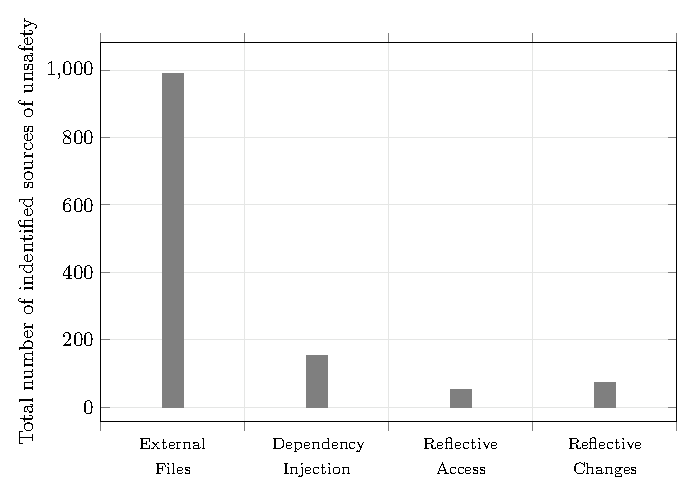
\includegraphics[scale=0.7]{./figures/pdf/commit_bar.pdf}
      \end{minipage}\hfill
      \begin{minipage}[c]{0.3\textwidth}
         \caption{Number of detected sources of unsafety.}
      \end{minipage}
   \end{figure}

   \itemNote{
      \item chart to show the composition of the detected sources of unsafety
      \item Majority of detected unsafety comes from external files
      \item Next biggest part is associated with dependency injection
   }
   \timer{17}
\end{frame}

\begin{subframe}[fragile]
   \frametitle{Results}
   \framesubtitle{Occurence of Sources of Unsafety in the Wild}
   \begin{figure}
      \begin{minipage}[c]{0.67\textwidth}
         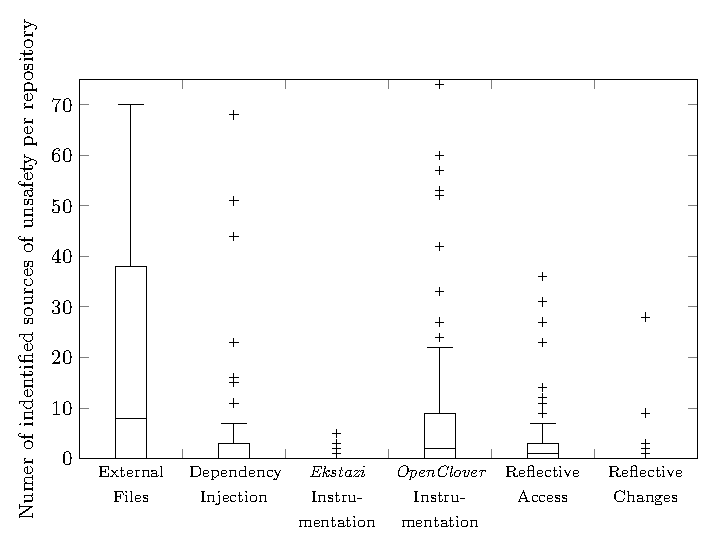
\includegraphics[scale=0.7]{./figures/pdf/box_plot.pdf}
      \end{minipage}\hfill
      \begin{minipage}[c]{0.3\textwidth}
         \caption{
            Sources of unsafety per repository (Removed outliers above 75 sources of unsafety. The full diagram is shown on the next slide.).
         }
      \end{minipage}
   \end{figure}
\end{subframe}

\begin{subframe}
   \frametitle{Results}
   \framesubtitle{Occurence of Sources of Unsafety in the Wild}
   \begin{figure}
      \begin{minipage}[c]{0.67\textwidth}
         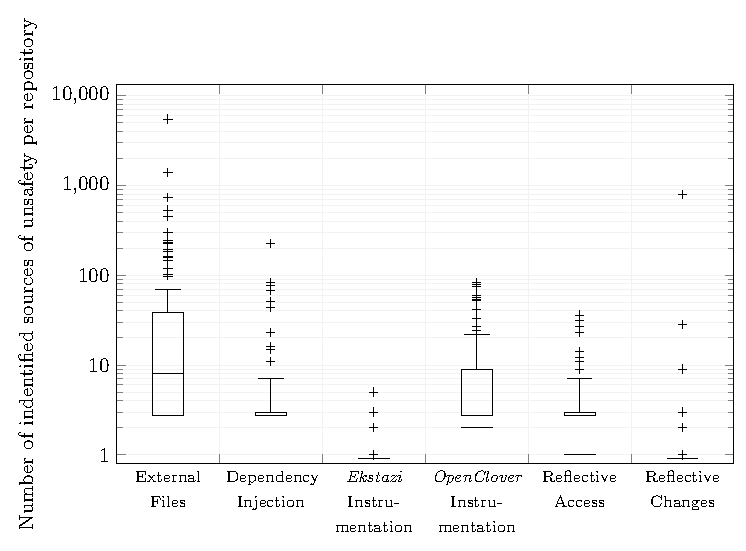
\includegraphics[scale=0.7]{./figures/pdf/box_plot_outliers.pdf}
      \end{minipage}\hfill
      \begin{minipage}[c]{0.3\textwidth}
         \caption{
            Sources of unsafety per scanned repository (Including all outliers).
         }
      \end{minipage}
   \end{figure}
   \itemNote{
      \item Box plot showing the number of sources of unsafety per repository
      \item Y-scale is logarithmic
      \item Big outliers for external files and reflective accesses
   }
\end{subframe}

\begin{frame}
   \centering\Huge
   Conclusions
   \timer{20}
\end{frame}

\section{Conclusions}
\begin{frame}
   \frametitle{Conclusion}
   \framesubtitle{The Alarming State of RTS for Java}
   \begin{itemize}
      \setlength\itemsep{1em}
      \item All examined RTS-tools act in an unsafe manner.
      \item Latest versions of the tools cannot be used as \textbf{safe} RTS-tools.
      \item \textbf{Safe} RTS for Java is possible though, but it is not easy.
   \end{itemize}
   \itemNote{
      \item We couldn't identify a suitable tool for safe RTS for Java.
      \item Although safety is theoretically possible, faulty implementations or methodological limitations can make RTS-tools unsafe.
      \item
   }
   \timer{20}
\end{frame}

\begin{frame}
   \frametitle{Conclusion}
   \framesubtitle{Maintenance of Research Projects}
   \begin{itemize}
      \setlength\itemsep{1em}
      \item Tools developed for research purposes are not maintained properly.
      \item Further research has to focus on improving existing tools.
   \end{itemize}
   \itemNote{
      \item We identified the common pattern that RTS-tools from research papers are not well maintained.
      \item  => Research should focus on improving existing solutions, rather than creating new, unmaintained solutions.
   }
   \timer{20}
\end{frame}


\begin{frame}
   \centering\Huge
   Thank you for your attention
\end{frame}

\backupbegin

\begin{frame}
   \centering\Huge
   Time for Questions
\end{frame}

\begin{frame}
   \centering\Huge
   Appendix
\end{frame}

% End Slides
\appendix

\begin{frame}[allowframebreaks]
   \frametitle{Bibliography}
   \printbibliography
\end{frame}

\begin{frame}
   \centering\Huge
   Backup Slides
\end{frame}

\appendsubframes

\backupend

\begin{frame}
   \centering
   \doclicenseThis
\end{frame}
\end{document}
